Die unterschiedlichen Teile des Lasers werden auf einer optischen Schiene aufgebaut. Ein Justierlaser dient der exakten
Ausrichtung aller Komponenten, sodass der Laser das Licht optimal verstärken kann. Mittig befindet sich das Laserrohr
mit dem Helium-Neon-Gasgemisch und links und rechts davon zwei Spiegel, die das Licht sehr gut reflektieren bzw. teilweise
durchlassen. Des Weiteren befinden sich Brewsterfenster an den Seiten des Laserrohrs, um das Licht zu polarisieren.
Am Rohr befinden sich außerdem zwei Elektroden, an die eine Spannung angelegt werden kann, um die Gasentladung im Rohr zu
erzeugen.
Für die unterschiedlichen Versuchsdurchführungen können verschiedene Komponenten zusätzlich eingebaut werden. Es stehen
ein Polarisationsfilter, ein Gitter, ein Draht und eine Photodiode zur Messung des Stroms zur Verfügung.

\begin{figure}[H]
  \centering
    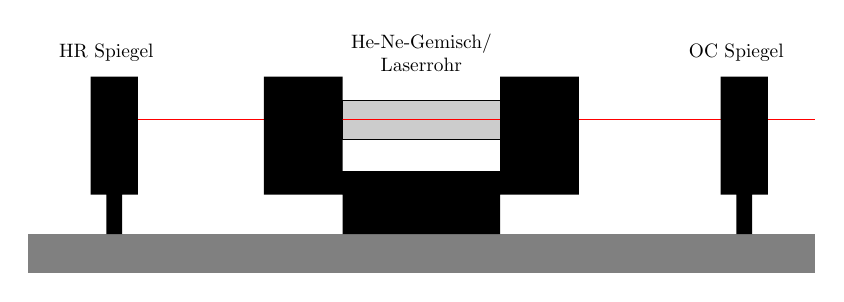
\begin{tikzpicture}
    \fill[white!50!black] (0,0)--(10,0)--(10,0.5)--(0,0.5)--cycle;
    \filldraw[fill=black!20!white] (4,2.2)--(6,2.2)--(6,1.7)--(4,1.7)--cycle;
    \node[scale=0.7,align=center] at (5,2.8) {He-Ne-Gemisch/\\Laserrohr};
    \draw[red] (1,1.95)--(10,1.95);

    \fill (1,0.5)--(1,1)--(0.8,1)--(0.8,2.5)--(1.4,2.5)--(1.4,1)--(1.2,1)--(1.2,0.5)--cycle;
    \node[scale=0.7] at (1,2.8) {HR Spiegel};
    \fill (9,0.5)--(9,1)--(8.8,1)--(8.8,2.5)--(9.4,2.5)--(9.4,1)--(9.2,1)--(9.2,0.5)--cycle;
    \node[scale=0.7] at (9,2.8) {OC Spiegel};

    \fill (4,0.5)--(4,1)--(3,1)--(3,2.5)--(4,2.5)--(4,1.3)--(6,1.3)--(6,2.5)--(7,2.5)--(7,1)--(6,1)--(6,0.5)--cycle;
    \end{tikzpicture}
  \caption{Skizze des Versuchsaufbaus}
  \label{fig:aufbau}
\end{figure}
